\section{Media di funzioni e Momenti di variabili continue}

\subsection{Media di funzioni di variabili aleatorie continue}

Sia $X \sim f_X(x)$ e sia $Y = g(X)$, con $\mathcal{Y} = g(\mathcal{X})$. Vogliamo estendere alle variabili continue il \textbf{Teorema Fondamentale per il calcolo della media} (LOTUS - Law of the Unconscious Statistician, vedi slide 60 e seguenti).
Il risultato principale - diretta derivazione del caso discreto - è che, qualunque sia $g(x)$:

\begin{equation}
\mathbb{E}[Y] = \mathbb{E}[g(X)] = \int_{\mathbb{R}} g(x)f_X(x) dx
\end{equation}

La dimostrazione formale ricalca il concetto di quantizzazione:
\begin{itemize}
    \item Definiamo una versione quantizzata di $X$ a $M$ livelli, $X^\Delta$, in modo del tutto analogo a quanto fatto per ricavare la media di variabili continue.
    \item A questa applichiamo la trasformazione $g(\cdot)$, ottenendo la variabile discreta $Y^\Delta = g(X^\Delta)$:
    \[ X^\Delta = x_i \in [i\Delta, (i+1)\Delta[ \implies i\Delta \le X < (i+1)\Delta \implies g(X^\Delta) = g(x_i) \]
    \item Il teorema quindi segue - se $g(x)f_X(x)$ è Riemann-integrabile - passando al limite per $\Delta \to 0$:
\end{itemize}

\begin{equation}
\mathbb{E}[Y] = \lim_{\Delta \to 0} \mathbb{E}[Y^\Delta] = \lim_{\Delta \to 0} \sum_{i=1}^{M} g(x_i) \underbrace{f_X(x_i)\Delta}_{\simeq \mathbb{P}(i\Delta \le X < (i+1)\Delta)} = \int_{\mathbb{R}} g(x)f_X(x) dx
\end{equation}

\subsection{Valore quadratico medio e varianza di variabili continue}

È a questo punto immediata la generalizzazione dei concetti introdotti per le variabili discrete a quelle continue. Data una variabile aleatoria $X \sim f_X(x), x \in \mathcal{X}$, con media $\mu_X = \mathbb{E}[X]$ definiamo:

\begin{itemize}
    \item \textbf{Il valore quadratico medio} (Mean Square) di $X$:
    \begin{equation}
    X_{rms}^2 = \mathbb{E}[X^2] = \int_{\mathbb{R}} x^2 f_X(x) dx
    \end{equation}
    
    \item \textbf{Il valore efficace} (root mean square, rms) di $X$:
    \begin{equation}
    X_{rms} = \sqrt{\mathbb{E}[X^2]} = \sqrt{\int_{\mathbb{R}} x^2 f_X(x) dx}
    \end{equation}
    
    \item \textbf{La varianza} di $X$:
    \begin{equation}
    \sigma_X^2 = \mathbb{E}[(X - \mu_X)^2] = \int_{\mathbb{R}} (x^2 + \mu_X^2 - 2x\mu_X) f_X(x) dx = X_{rms}^2 - \mu_X^2
    \end{equation}
    
    \item \textbf{La deviazione standard} di $X$:
    \begin{equation}
    \sigma_X = \sqrt{\sigma_X^2} = \sqrt{\mathbb{E}[X^2] - \mu_X^2} = \sqrt{X_{rms}^2 - \mu_X^2}
    \end{equation}
\end{itemize}

\textit{Nota: Tutte le proprietà studiate in precedenza per media e varianza (es. linearità) ovviamente valgono anche per le variabili continue.}

\subsection{Calcolo dei Momenti per le Distribuzioni Notevoli}

Di seguito vengono riportate le dimostrazioni per il calcolo della media, del valore quadratico medio e della varianza per le distribuzioni continue più comuni.

\subsubsection{Sia $X \sim \mathcal{U}(a, b)$}

$X$ ha una probabilità costante nell'intervallo $[a, b]$ e $0$ altrove, la sua PDF è:
\[ f_X(x) = \frac{1}{b-a} \quad \text{per} \quad a \le x \le b \]

Per calcolare $\mathbb{E}[X]$ usiamo la definizione:
\begin{align}
\mathbb{E}[X] &= \int_{-\infty}^{+\infty} x f_X(x) dx = \int_{a}^{b} x \frac{1}{b-a} dx = \frac{1}{b-a} \int_{a}^{b} x dx = \frac{1}{b-a} \left[ \frac{x^2}{2} \right]_{a}^{b} \nonumber \\
&= \frac{1}{b-a} \left( \frac{b^2}{2} - \frac{a^2}{2} \right) = \frac{1}{2} \cdot \frac{b^2 - a^2}{b-a} = \frac{1}{2} \frac{(b-a)(b+a)}{b-a} \nonumber \\
\implies \mathbb{E}[X] &= \frac{a+b}{2}
\end{align}

Per calcolare la $Var(X)$ dobbiamo prima trovare $\mathbb{E}[X^2]$:
\begin{align}
\mathbb{E}[X^2] &= \int_{-\infty}^{+\infty} x^2 f_X(x) dx = \int_{a}^{b} x^2 \frac{1}{b-a} dx = \frac{1}{b-a} \left[ \frac{x^3}{3} \right]_{a}^{b} = \frac{1}{b-a} \frac{1}{3} (b^3 - a^3) \nonumber \\
&= \frac{1}{3} \frac{b^3 - a^3}{b-a} = \frac{1}{3} \frac{(b-a)(b^2 + ab + a^2)}{b-a} \nonumber \\
\implies \mathbb{E}[X^2] &= \frac{b^2 + ab + a^2}{3}
\end{align}

Ora calcoliamo la varianza:
\begin{align}
\sigma^2 &= \mathbb{E}[X^2] - \mathbb{E}^2[X] = \frac{a^2 + ab + b^2}{3} - \left(\frac{a+b}{2}\right)^2 = \frac{a^2 + ab + b^2}{3} - \frac{a^2 + 2ab + b^2}{4} \nonumber \\
&= \frac{4a^2 + 4ab + 4b^2 - 3a^2 - 6ab - 3b^2}{12} = \frac{a^2 - 2ab + b^2}{12} \nonumber \\
\implies \sigma^2 &= \frac{(b-a)^2}{12}
\end{align}


\subsubsection{Sia $X \sim \mathcal{E}(\lambda)$}

Ricordiamo che la variabile esponenziale monolatera ha la seguente PDF:
\[ f_X(x) = \lambda e^{-\lambda x} u(x) \qquad u(x) = \begin{cases} 1 & x \ge 0 \\ 0 & x < 0 \end{cases} \]

\begin{equation}
\mathbb{E}[X] = \int_{-\infty}^{+\infty} x f_X(x) dx = \int_{0}^{+\infty} x \cdot \lambda e^{-\lambda x} dx
\end{equation}

Facciamo una sostituzione: sia $t = \lambda x \implies x = \frac{t}{\lambda} \implies dx = \frac{dt}{\lambda}$. \\
\textit{Osservazione sui limiti:} Se $x=0 \implies t=0$ e se $x \to +\infty \implies t \to +\infty$.

\begin{equation}
\int_{0}^{+\infty} \frac{t}{\lambda} \lambda e^{-t} \frac{dt}{\lambda} = \frac{1}{\lambda} \int_{0}^{+\infty} \underbrace{t}_{u} \underbrace{e^{-t} dt}_{dv}
\end{equation}

Risolviamo per parti: $\int u dv = u \cdot v - \int v du$.
\[ u = t \implies du = 1 \cdot dt \]
\[ dv = e^{-t} dt \implies v = \int e^{-t} dt = -e^{-t} \]

\[ t \cdot (-e^{-t}) - \int -e^{-t} dt = -t e^{-t} - e^{-t} = -e^{-t}(t + 1) \quad \longleftarrow \text{PRIMITIVA} \]

Valutiamo la primitiva in $0$ e $+\infty$:
\[ \left| -(t+1)e^{-t} \right|_0^{+\infty} = \lim_{b \to +\infty} \left| -(t+1)e^{-t} \right|_0^{b} = \lim_{t \to +\infty} \frac{-(t+1)}{e^t} - \left( -(0+1) \cdot e^0 \right) = 0 - (-1) = 1 \]

Quindi:
\begin{equation}
\mathbb{E}[X] = \int_{0}^{+\infty} x \cdot \lambda e^{-\lambda x} dx = \frac{1}{\lambda} \int_{0}^{+\infty} t e^{-t} dt = \frac{1}{\lambda} \cdot 1 = \frac{1}{\lambda}
\end{equation}

Passiamo al calcolo di $Var(X)$.
\begin{equation}
\mathbb{E}[X^2] = \int_{\mathbb{R}} x^2 f_X(x) = \int_{0}^{+\infty} \underbrace{x^2}_{u} \underbrace{\lambda e^{-\lambda x} dx}_{dv}
\end{equation}

Integriamo per parti:
\[ u = x^2 \implies du = 2x \implies du = 2x dx \]
\[ dv = \lambda e^{-\lambda x} dx \implies \int dv = \int \lambda e^{-\lambda x} dx \implies \text{per sost. } y = -\lambda x \implies dy = -\lambda dx \implies dx = -\frac{dy}{\lambda} \]
\[ \dots \implies \lambda \int e^y \left(-\frac{dy}{\lambda}\right) = - \int e^y dy = -e^y + C \implies v = -e^{-\lambda x} \]

Applicando la formula dell'integrazione per parti:
\begin{equation}
x^2 (-e^{-\lambda x}) - \int -e^{-\lambda x} \cdot 2x dx = \left[ -x^2 e^{-\lambda x} \right]_0^{+\infty} + 2 \int_{0}^{+\infty} x e^{-\lambda x} dx
\end{equation}

Ora abbiamo due strade: integrare di nuovo oppure moltiplicare e dividere per $\lambda$ e osservare che $\lambda \int x e^{-\lambda x} dx$ è l'$\mathbb{E}[X]$ che abbiamo già calcolato.

\begin{equation}
\left[ -x^2 e^{-\lambda x} \right]_0^{+\infty} + \frac{2}{\lambda} \int_{0}^{+\infty} x \lambda e^{-\lambda x} dx = \left[ \frac{-x^2}{e^{\lambda x}} \right]_0^{+\infty} + \frac{2}{\lambda} \cdot \overbrace{ \frac{1}{\lambda} }^{\mathbb{E}[X]} = (0 - 0) + \frac{2}{\lambda^2}
\end{equation}

Quindi $\mathbb{E}[X^2] = \frac{2}{\lambda^2}$.

La varianza sarà:
\begin{equation}
\sigma^2 = \mathbb{E}[X^2] - \mathbb{E}^2[X] = \frac{2}{\lambda^2} - \left(\frac{1}{\lambda}\right)^2 = \frac{2}{\lambda^2} - \frac{1}{\lambda^2} = \frac{1}{\lambda^2}
\end{equation}


\subsubsection{Sia $X \sim \mathcal{L}(\lambda)$}

La PDF è $f_X(x) = \frac{\lambda}{2} e^{-\lambda |x|} \quad \forall x \in \mathbb{R}$.
Data la presenza del valore assoluto $|x|$, la funzione è perfettamente simmetrica rispetto all'asse $y$, è una funzione pari.

\begin{equation}
\mathbb{E}[X] = \int_{-\infty}^{+\infty} x f_X(x) dx = \frac{\lambda}{2} \int_{-\infty}^{+\infty} x \cdot e^{-\lambda |x|} dx
\end{equation}

\begin{itemize}
    \item $g(x) = x$ è una funzione dispari ($g(-x) = -g(x)$).
    \item $f_X(x) = e^{-\lambda |x|}$ è pari ($f(-x) = f(x)$).
    \item Il prodotto tra una funzione pari ed una dispari è una funzione dispari.
    \item L'integrale definito su un intervallo simmetrico di una funzione dispari è $0$.
\end{itemize}
Quindi $\mathbb{E}[X] = 0$.

Calcoliamo il valore quadratico medio:
\begin{equation}
\mathbb{E}[X^2] = \int_{\mathbb{R}} x^2 \frac{\lambda}{2} e^{-\lambda |x|} dx
\end{equation}
\begin{itemize}
    \item $x^2$ è pari.
    \item $e^{-\lambda |x|}$ è pari.
    \item La risultante è pari.
\end{itemize}

Essendo integranda pari su dominio simmetrico, il calcolo si riduce a:
\begin{equation}
2 \cdot \int_{0}^{+\infty} x^2 \frac{\lambda}{2} e^{-\lambda x} dx = \int_{0}^{+\infty} x^2 \lambda e^{-\lambda x} dx
\end{equation}

Ma questa è esattamente $\mathbb{E}[X^2]$ per $X \sim \mathcal{E}(\lambda)$ esponenziale (che abbiamo appena calcolato e vale $2/\lambda^2$). Quindi:
\begin{equation}
\mathbb{E}[X^2] = \frac{2}{\lambda^2}
\end{equation}

La varianza risulta:
\begin{equation}
\sigma^2 = \mathbb{E}[X^2] - \mathbb{E}^2[X] = \frac{2}{\lambda^2} - 0 = \frac{2}{\lambda^2}
\end{equation}

\subsubsection{Sia $X \sim \mathcal{C}(a, b)$}
Come anticipato nella teoria, a causa delle code pesanti dell'integranda, per la distribuzione di Cauchy \textbf{non esistono} né la media, né la varianza e, di conseguenza, nemmeno il valore rms o la deviazione standard.

\section{Variabili Aleatorie Continue Multiple}

Per studiare come diverse grandezze interagiscono tra loro, ci servono strumenti come la densità congiunta per capire se due variabili sono legate. Per farlo dobbiamo definire una coppia di variabili aleatorie, proprio come nel caso discreto.

In perfetta analogia con quanto fatto per le variabili discrete, una coppia di variabili continue (o variabile doppia) è definita nella forma di una mappatura vettoriale:

\begin{equation}
X, Y : \omega \in \Omega \longrightarrow (X(\omega), Y(\omega)) \in \mathcal{X} \times \mathcal{Y} \subseteq \mathbb{R}^2
\end{equation}

dove $\mathcal{X}$ e $\mathcal{Y}$ sono gli alfabeti (i supporti) di $X$ e di $Y$ rispettivamente.

Analogamente, date tre variabili aleatorie (a questo punto non importa più se tutte continue o meno) avremo:
\begin{equation}
X, Y, Z : \omega \in \Omega \longrightarrow (X(\omega), Y(\omega), Z(\omega)) \in \mathcal{X} \times \mathcal{Y} \times \mathcal{Z} \subseteq \mathbb{R}^3
\end{equation}

In generale, date $m$ variabili aleatorie definiamo una $m$-upla aleatoria. Sia $X_i \in \mathcal{X}_i \subseteq \mathbb{R}$, avremo:
\begin{equation}
X_1, X_2, \dots, X_m : \omega \in \Omega \longrightarrow (X_1(\omega), \dots, X_m(\omega)) \in \mathcal{X}_1 \times \dots \times \mathcal{X}_m \subseteq \mathbb{R}^m
\end{equation}

\subsection{Visualizzazione e il Problema del Continuo}

Siano $X$ e $Y$ due variabili aleatorie continue. Visualizziamole sul piano cartesiano:

\begin{center}
\begin{tikzpicture}
    \begin{axis}[
        width=8cm, height=6cm,
        axis lines=middle,
        xlabel={$x$}, ylabel={$y$},
        xmin=-0.5, xmax=5,
        ymin=-0.5, ymax=5,
        xtick=\empty, ytick=\empty,
        every axis x label/.style={at={(ticklabel* cs:1.05)}, anchor=west,},
        every axis y label/.style={at={(ticklabel* cs:1.05)}, anchor=south,}
    ]
        % Punti sparsi per simulare il disegno a mano
        \addplot[mark=*, only marks, mark size=1pt, gray] coordinates {
            (1.5, 2.1) (2.1, 1.8) (1.2, 3.0) (2.8, 2.5) (3.2, 1.5) 
            (2.5, 3.5) (3.8, 2.8) (1.8, 1.2) (3.5, 3.8) (4.2, 2.0)
            (2.2, 2.7) (3.0, 3.1) (1.5, 3.5)
        };
        
        % Punto evidenziato in rosso
        \addplot[mark=*, only marks, mark size=2pt, red] coordinates {(2.2, 2.7)} 
        node[anchor=south west, text=black] {$(x,y)$};
        
        % Linee tratteggiate generiche per formare un'area di densità
        \draw[dashed, gray] (axis cs: 1,1) rectangle (axis cs: 4.5,4);
    \end{axis}
\end{tikzpicture}
\end{center}

La coppia $(x,y)$ rappresenta una specifica combinazione dei valori assunti da $X$ e $Y$. 

Però ricordiamo che nel caso continuo esistono infiniti punti nel piano. Pertanto, chiedere \textit{"qual è la probabilità..."}

\vspace{0.5cm}

\subsubsection*{Approfondimento: Dal punto all'Area (Densità Congiunta)}

Completiamo il ragionamento interrotto negli appunti: chiedere \textit{"qual è la probabilità di ottenere esattamente la specifica combinazione di numeri $(x,y)$?"} porta a un problema matematico. Essendo i punti nel piano infiniti e continui, \textbf{la probabilità di centrare un singolo punto esatto è sempre nulla}:
\begin{equation}
\mathbb{P}(X=x, Y=y) = 0
\end{equation}

Per questo motivo, l'immagine dei "pallini" (scatter plot) è utile per l'intuizione iniziale (e corrisponde al caso delle variabili \textit{discrete} doppie), ma smette di funzionare per il caso continuo. 

Per le variabili continue, la probabilità non risiede nei singoli punti, ma nelle \textbf{Aree}. 
Invece di chiederci la probabilità di un punto, dobbiamo chiederci la probabilità che la coppia cada all'interno di un certo rettangolo infinitesimo di base $dx$ e altezza $dy$. 

Per fare questo, passeremo dall'avere una curva 2D (come la $f_X(x)$) ad avere una \textbf{superficie 3D}: la Funzione di Densità di Probabilità Congiunta $f_{XY}(x,y)$. La probabilità non sarà più un'area sottesa a una curva, ma un \textbf{Volume} sotteso a questa superficie tridimensionale.

... chiedere \textit{"qual è la probabilità} in un punto $(x,y)$" porterebbe alla risposta 0.

\subsection{Definizione della PDF Congiunta}

Come già abbiamo fatto, consideriamo un intorno del punto che definiamo con un rettangolo/quadrato di altezza $\Delta y$ e larghezza $\Delta x$.

\begin{center}
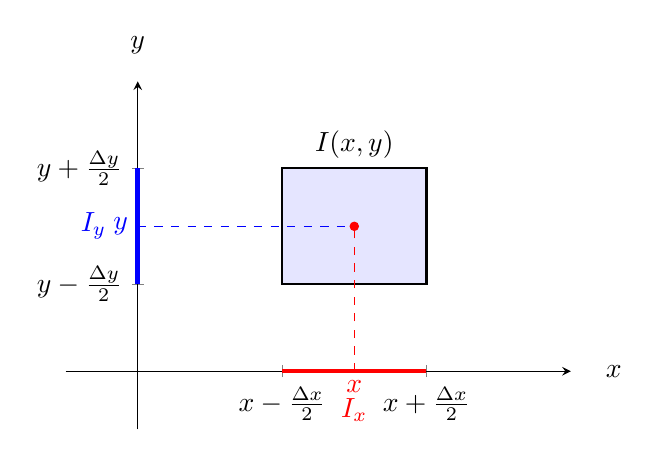
\begin{tikzpicture}
    \begin{axis}[
        width=8cm, height=6cm,
        axis lines=middle,
        xlabel={$x$}, ylabel={$y$},
        xmin=-1, xmax=6,
        ymin=-1, ymax=5,
        xtick={2, 4},
        xticklabels={$x-\frac{\Delta x}{2}$, $x+\frac{\Delta x}{2}$},
        ytick={1.5, 3.5},
        yticklabels={$y-\frac{\Delta y}{2}$, $y+\frac{\Delta y}{2}$},
        every axis x label/.style={at={(ticklabel* cs:1.05)}, anchor=west,},
        every axis y label/.style={at={(ticklabel* cs:1.05)}, anchor=south,}
    ]
        % Area del quadrato
        \addplot[fill=blue!10, draw=none] coordinates {(2,1.5) (4,1.5) (4,3.5) (2,3.5)};
        
        % Linee del quadrato
        \draw[thick, black] (axis cs:2,1.5) rectangle (axis cs:4,3.5);
        
        % Punto centrale
        \addplot[mark=*, only marks, mark size=1.5pt, red] coordinates {(3, 2.5)};
        
        % Linee tratteggiate verso gli assi
        \draw[dashed, blue] (axis cs:0,2.5) -- (axis cs:3,2.5);
        \draw[dashed, red] (axis cs:3,0) -- (axis cs:3,2.5);
        \node[anchor=east, text=blue] at (axis cs: 0, 2.5) {$y$};
        \node[anchor=north, text=red] at (axis cs: 3, 0) {$x$};
        
        % Label dell'intervallo
        \node[anchor=south] at (axis cs: 3, 3.5) {$I(x,y)$};
        
        % Intervalli sugli assi evidenziati
        \draw[ultra thick, red] (axis cs:2,0) -- (axis cs:4,0);
        \node[anchor=north, text=red] at (axis cs: 3, -0.3) {$I_x$};
        
        \draw[ultra thick, blue] (axis cs:0,1.5) -- (axis cs:0,3.5);
        \node[anchor=east, text=blue] at (axis cs: -0.3, 2.5) {$I_y$};
    \end{axis}
\end{tikzpicture}
\end{center}

Quanto più $\Delta x$ e $\Delta y$ diventano piccoli, tanto più il quadrato approssima bene il punto $(x,y)$.
Definiamo la PDF congiunta delle variabili aleatorie continue $X$ e $Y$:

\begin{equation}
f_{X,Y}(x,y) = \lim_{\Delta x \to 0} \lim_{\Delta y \to 0} \frac{\mathbb{P}\left(\left\{x - \frac{\Delta x}{2} \le X \le x + \frac{\Delta x}{2}\right\} \cap \left\{y - \frac{\Delta y}{2} \le Y \le y + \frac{\Delta y}{2}\right\}\right)}{\Delta x \Delta y}
\end{equation}

Che in modo compatto si scrive:
\begin{equation}
f_{X,Y}(x,y) = \lim_{\Delta x \to 0} \lim_{\Delta y \to 0} \frac{P_{X,Y}(x,y; \Delta x, \Delta y)}{\Delta x \Delta y}
\end{equation}

L'intersezione rappresenta tutti i punti nel quadrato. Vogliamo la probabilità di appartenere a questo intervallo $I(x,y)$ quando $\Delta x$ e $\Delta y$ sono infinitesimi.

\subsection{Dal Volume alla Probabilità}

\begin{center}
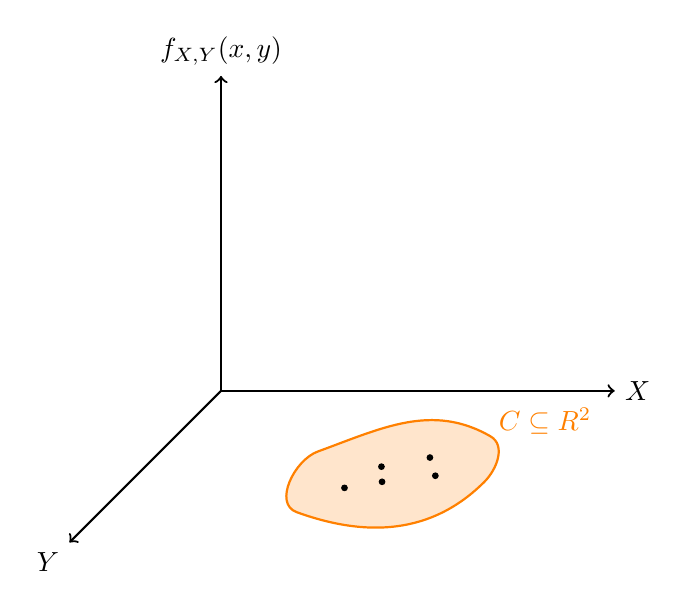
\begin{tikzpicture}
    % Assi 3D
    \draw[->, thick] (0,0,0) -- (5,0,0) node[right] {$X$};
    \draw[->, thick] (0,0,0) -- (0,4,0) node[above] {$f_{X,Y}(x,y)$};
    \draw[->, thick] (0,0,0) -- (0,0,5) node[below left] {$Y$};
    
    % Dominio C nel piano XY (che è XZ in TikZ 3D standard, quindi usiamo coordinate piatte)
    \draw[fill=orange!20, draw=orange, thick] (2,0,2) to[out=20,in=150] (4,0,1.5) to[out=-30,in=45] (4.5,0,3) to[out=225,in=-20] (2.5,0,4) to[out=160,in=200] (2,0,2);
    
    \node[orange] at (4.5,0,1) {$C \subseteq \mathbb{R}^2$};
    
    % Punti nel dominio
    \filldraw[black] (3,0,2.5) circle (1pt);
    \filldraw[black] (3.5,0,2.2) circle (1pt);
    \filldraw[black] (3.2,0,3) circle (1pt);
    \filldraw[black] (2.8,0,3.2) circle (1pt);
    \filldraw[black] (3.8,0,2.8) circle (1pt);
\end{tikzpicture}
\end{center}

L'asse $z$ rappresenta il valore restituito dalla funzione congiunta $f_{X,Y}(x,y)$. Otteniamo una superficie tridimensionale, i punti con il valore $z$ maggiore sono i punti $(x,y)$ più densi, ovvero più probabili da osservare se prendiamo un piccolo intervallo attorno all'asse.

Se moltiplichiamo l'area del rettangolino $\Delta x \Delta y$ per l'altezza della funzione rispetto a quel punto otteniamo il volume:

\begin{equation}
\text{Volume} \approx f_{X,Y}(x,y) \cdot \Delta x \Delta y
\end{equation}

Il volume rappresenta proprio la probabilità che la coppia $(x,y)$ cada in quel rettangolino.

Ipotizziamo di definire una regione $C$ del piano cartesiano che rappresenta una condizione per $X$ e $Y$. \textit{"Qual è la probabilità che $(x,y)$ cada dentro $C$?"} ovvero $\mathbb{P}((X,Y) \in C)$.

Poiché la densità è stata ottenuta dividendo la probabilità per un'area infinitesima, possiamo riottenere la probabilità moltiplicandola per la densità per un'area infinitesima ($dx dy$), sommandola per tutti questi elementi:

\begin{equation}
\mathbb{P}((X,Y) \in C) = \iint_C f_{X,Y}(x,y) dx dy
\end{equation}

Sommiamo gli infiniti "volumetti" sino ad ottenere tutto il volume di $C$.

\subsubsection*{Vincoli Costitutivi (Proprietà)}
Dalla definizione geometrica e analitica osserviamo che:
\begin{itemize}
    \item \textbf{Non negatività:} $f_{X,Y}(x,y) \ge 0 \quad \forall (x,y) \in \mathbb{R}^2$. Non possiamo sprofondare sotto il piano $XY$. Non esistono volumi (probabilità) negativi.
    \item \textbf{Integrale Unitario:} L'integrale doppio su $\mathbb{R}^2$ è uguale a 1.
    \begin{equation}
    \iint_{\mathbb{R}^2} f_{X,Y}(x,y) dx dy = \int_{-\infty}^{+\infty} \int_{-\infty}^{+\infty} f_{X,Y}(x,y) dx dy = \mathbb{P}((X,Y) \in \mathbb{R}^2) = 1
    \end{equation}
\end{itemize}

\subsection{Densità Marginali (Proprietà di Marginalizzazione)}

Cosa significa calcolare la densità marginale $f_X(x)$?
Significa che ti interessa sapere come si comporta \textbf{solo} la variabile $X$, ignorando completamente l'esito della variabile $Y$.

\begin{equation}
\int_{\mathbb{R}} f_{X,Y}(x,y) dy = f_X(x)
\end{equation}

In pratica significa \textbf{proiettare} contro la "parete" dell'asse $X$ la funzione 3D. Per ogni punto $x$, stai sommando tutta la probabilità lungo la linea dell'asse $Y$. Specularmente, per trovare la marginale di $Y$: $\int_{\mathbb{R}} f_{X,Y}(x,y) dx = f_Y(y)$.

\begin{center}
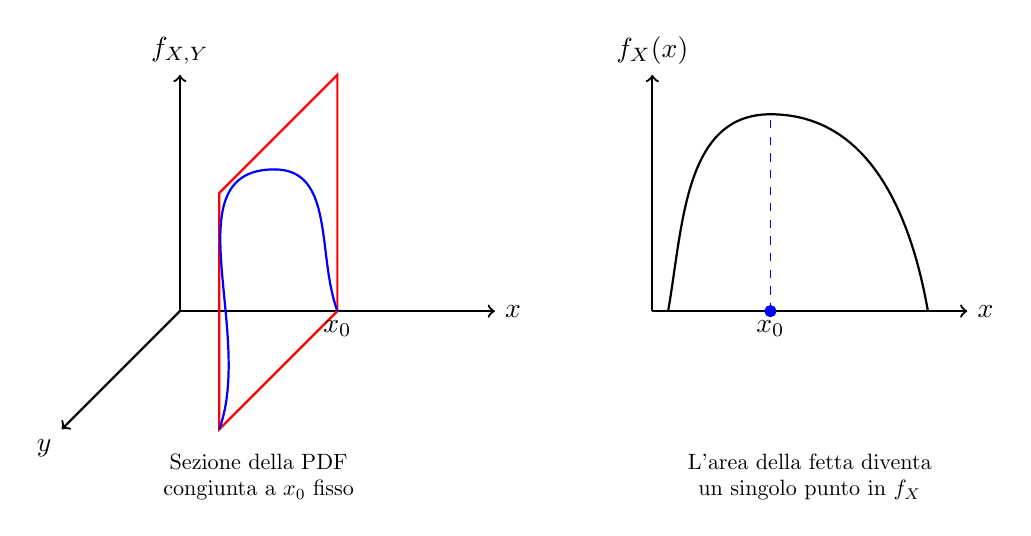
\begin{tikzpicture}
    % Asse 3D per mostrare la fetta
    \begin{scope}[shift={(0,0)}]
        \draw[->, thick] (0,0) -- (4,0) node[right] {$x$};
        \draw[->, thick] (0,0) -- (0,3) node[above] {$f_{X,Y}$};
        \draw[->, thick] (0,0) -- (-1.5,-1.5) node[below left] {$y$};
        
        % Piano proiettivo a x fisso
        \draw[draw=red, thick] (2,0) -- (0.5,-1.5) -- (0.5, 1.5) -- (2,3) -- cycle;
        
        % Curva sulla fetta
        \draw[thick, blue, smooth] (2,0) to[out=110, in=0] (1.2, 1.8) to[out=180, in=70] (0.5, -1.5);
        \node[anchor=north] at (2,0) {$x_0$};
        
        \node[anchor=south, align=center, scale=0.8] at (1, -2.5) {Sezione della PDF\\congiunta a $x_0$ fisso};
    \end{scope}
    
    % Asse 2D per mostrare la proiezione
    \begin{scope}[shift={(6,0)}]
        \draw[->, thick] (0,0) -- (4,0) node[right] {$x$};
        \draw[->, thick] (0,0) -- (0,3) node[above] {$f_X(x)$};
        
        % Curva marginale
        \draw[thick, black, smooth] (0.2,0) to[out=80,in=180] (1.5, 2.5) to[out=0,in=100] (3.5, 0);
        
        % Punto proiettato
        \draw[dashed, blue] (1.5,0) -- (1.5,2.5);
        \filldraw[blue] (1.5,0) circle (2pt) node[below, text=black] {$x_0$};
        
        \node[anchor=south, align=center, scale=0.8] at (2, -2.5) {L'area della fetta diventa\\un singolo punto in $f_X$};
    \end{scope}
\end{tikzpicture}
\end{center}

\textbf{Attenzione:} Se hai la PDF congiunta puoi proiettare sugli assi e ottenere le marginali. Se hai le marginali \textbf{NON puoi dedurre} la PDF congiunta (caratterizzare congiuntamente significa anche caratterizzarle marginalmente, mentre il viceversa non è necessariamente vero).

\subsubsection*{Dimostrazione della Marginalizzazione tramite CDF}

Per dimostrare la marginalizzazione dobbiamo introdurre la funzione di ripartizione marginale di $X$: $F_X(x) = \mathbb{P}(X \le x)$.
Ignorando $Y$, questo equivale a dire che $Y$ può assumere qualsiasi valore tra $-\infty$ e $+\infty$:
\begin{equation}
F_X(x) = \mathbb{P}(X \le x, -\infty \le Y \le +\infty)
\end{equation}

Per calcolare questa probabilità integriamo la densità congiunta sulla regione di interesse:
\begin{equation}
F_X(x) = \int_{-\infty}^{x} \left( \int_{-\infty}^{+\infty} f_{X,Y}(u,y) dy \right) du
\end{equation}

Per definizione la PDF è la derivata della CDF: $f_X(x) = \frac{d F_X(x)}{dx}$. Deriviamo a destra e a sinistra:
\begin{align}
f_X(x) &= \frac{d}{dx} \left[ \int_{-\infty}^{x} \left( \int_{-\infty}^{+\infty} f_{X,Y}(u,y) dy \right) du \right] \nonumber \\
&= \int_{-\infty}^{+\infty} f_{X,Y}(x,y) dy \nonumber \\
\implies f_X(x) &= \int_{\mathbb{R}} f_{X,Y}(x,y) dy
\end{align}

\subsection{Funzione di Ripartizione Congiunta e Indipendenza}

Definiamo CDF congiunta:
\begin{equation}
F_{X,Y}(x,y) = \mathbb{P}(X \le x, Y \le y)
\end{equation}

\subsubsection*{Indipendenza Statistica}
Due variabili aleatorie sono \textbf{indipendenti} se e solo se la loro caratterizzazione congiunta è pari al prodotto delle caratterizzazioni marginali:

\begin{equation}
f_{X,Y}(x,y) = f_X(x) \cdot f_Y(y) \iff F_{X,Y}(x,y) = F_X(x) \cdot F_Y(y)
\end{equation}

Più in generale, se abbiamo una $m$-upla aleatoria $X_i \sim f_{X_i}(x)$ con $x \in \mathcal{X}_i$, allora esse sono mutuamente indipendenti se e solo se:
\begin{equation}
f_{X_1, \dots, X_m}(x_1, \dots, x_m) = \prod_{i=1}^{m} f_{X_i}(x_i), \qquad (x_1, \dots, x_m) \in \mathbb{R}^m
\end{equation}
\subsection{Le PDF Condizionate}

Ipotizziamo di conoscere già l'esito ($y$) della variabile aleatoria $Y$. È come se fissassimo $Y$, e vogliamo sapere come si comporta $X$ sotto questa condizione.

Ricordiamo la definizione classica della probabilità condizionata (Teorema di Bayes per gli eventi):
\begin{equation}
\mathbb{P}(A|B) = \frac{\mathbb{P}(A \cap B)}{\mathbb{P}(B)}
\end{equation}

Traduciamo questa formula nel mondo delle variabili aleatorie continue, definendo gli eventi tramite gli intorni:
\begin{itemize}
    \item L'evento $A$ è \textit{"$X$ cade nell'intervallo $\Delta x$"} (ovvero $X \in I_x$).
    \item L'evento $B$ è \textit{"$Y$ cade nell'intervallo $\Delta y$"} (ovvero $Y \in I_y$).
\end{itemize}

L'intersezione $\mathbb{P}(X \in I_x \cap Y \in I_y)$ è data dalla probabilità congiunta $P_{X,Y}(x,y; \Delta x, \Delta y)$.
Il denominatore è la probabilità marginale di $Y$, ovvero la probabilità di "cadere nella striscia" orizzontale definita da $\Delta y$: $P_Y(y; \Delta y)$.

\begin{center}
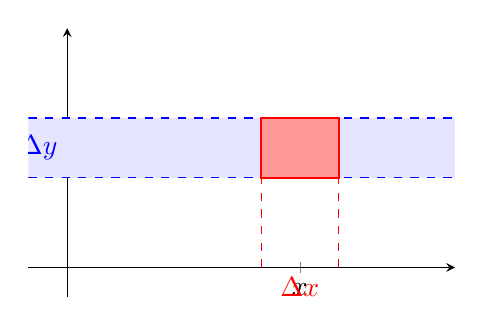
\begin{tikzpicture}
    \begin{axis}[
        width=7cm, height=5cm,
        axis lines=middle,
        xmin=-0.5, xmax=5,
        ymin=-0.5, ymax=4,
        xtick={3},
        xticklabels={$x$},
        ytick={2},
        yticklabels={$y$},
        xlabel={}, ylabel={},
        every axis x label/.style={at={(ticklabel* cs:1.05)}, anchor=west,},
        every axis y label/.style={at={(ticklabel* cs:1.05)}, anchor=south,}
    ]
        % Striscia orizzontale per Y
        \fill[blue!10] (-0.5, 1.5) rectangle (5, 2.5);
        \draw[dashed, blue] (-0.5, 1.5) -- (5, 1.5);
        \draw[dashed, blue] (-0.5, 2.5) -- (5, 2.5);
        \node[blue, anchor=east] at (0, 2) {$\Delta y$};
        
        % Rettangolino intersezione per X e Y
        \fill[red!40] (2.5, 1.5) rectangle (3.5, 2.5);
        \draw[thick, red] (2.5, 1.5) rectangle (3.5, 2.5);
        \draw[dashed, red] (2.5, 0) -- (2.5, 1.5);
        \draw[dashed, red] (3.5, 0) -- (3.5, 1.5);
        \node[red, anchor=north] at (3, 0) {$\Delta x$};
        
    \end{axis}
\end{tikzpicture}
\end{center}

Se sommiamo le densità di tutti questi rettangolini rossi lungo l'asse $x$, otteniamo la densità di probabilità marginale di $Y$ nel punto $y$, ovvero $f_Y(y)$.

Per passare dalla probabilità alla \textbf{densità} rispetto a $X$, dobbiamo dividere per l'intervallo $\Delta x$ e farlo tendere a $0$. Formalizzando analiticamente (come da slide):

\begin{equation}
\mathbb{P}\left(\left. x - \frac{\Delta x}{2} \le X \le x + \frac{\Delta x}{2} \right| y - \frac{\Delta y}{2} \le Y \le y + \frac{\Delta y}{2} \right) = \frac{P_{X,Y}(x,y; \Delta x, \Delta y)}{P_Y(y; \Delta y)}
\end{equation}

Pertanto la densità di $X$ condizionata all'evento $\left\{y - \frac{\Delta y}{2} \le Y \le y + \frac{\Delta y}{2}\right\}$ si ottiene dividendo per $\Delta x$ e applicando il limite:
\begin{equation}
\lim_{\Delta x \to 0} \frac{P_{X,Y}(x,y; \Delta x, \Delta y)}{\Delta x P_Y(y; \Delta y)} = f_{X | \left\{y - \frac{\Delta y}{2} \le Y \le y + \frac{\Delta y}{2}\right\}} (x)
\end{equation}

Facendo dunque tendere anche $\Delta y$ a zero (assumendo la condizione puntuale $Y=y$), otteniamo la definizione fondamentale della \textbf{PDF Condizionata}:

\begin{equation}
\boxed{ f_{X|Y}(x|y) = \lim_{\Delta x \to 0} \lim_{\Delta y \to 0} \frac{P_{X,Y}(x,y; \Delta x, \Delta y)}{P_Y(y; \Delta y)} = \frac{f_{X,Y}(x,y)}{f_Y(y)} }
\end{equation}

Questo risultato, come c'era da attendersi, riproduce l'analoga definizione vista per la PMF condizionale del caso discreto. D'altronde, essa stessa è una densità a tutti gli effetti.

\subsubsection{Proprietà delle PDF Condizionate}
Data l'analogia con le variabili discrete, tutte le proprietà si estendono alle PDF condizionali:

\begin{itemize}
    \item \textbf{Validità come PDF:} $f_{X|Y}(x|y)$, se $y$ resta fisso e $x$ varia in $\mathcal{X}$, è una densità di probabilità a tutti gli effetti. Soddisfa i vincoli costitutivi:
    \begin{equation}
    f_{X|Y}(x|y) \ge 0 \qquad \text{e} \qquad \int_{\mathbb{R}} f_{X|Y}(x|y) dx = 1
    \end{equation}
    
    \item \textbf{Legge della probabilità totale per le PDF:} 
    Possiamo ricavare le marginali saturando (integrando) il prodotto tra la PDF condizionata e la PDF marginale della variabile condizionante:
    \begin{align}
    f_X(x) &= \int_{\mathbb{R}} f_{X,Y}(x,y) dy = \int_{\mathbb{R}} f_{X|Y}(x|y) f_Y(y) dy \\
    f_Y(y) &= \int_{\mathbb{R}} f_{X,Y}(x,y) dx = \int_{\mathbb{R}} f_{Y|X}(y|x) f_X(x) dx
    \end{align}

    \item \textbf{Leggi della probabilità composta e Teorema di Bayes per le densità:}
    \begin{equation}
    f_{X,Y}(x,y) = f_Y(y)f_{X|Y}(x|y) = f_X(x)f_{Y|X}(y|x) \implies f_{Y|X}(y|x) = \frac{f_Y(y)f_{X|Y}(x|y)}{f_X(x)}
    \end{equation}
\end{itemize}

\subsection{Altre estensioni per Variabili Multiple}

Come nel caso discreto, i concetti legati al valore atteso si estendono naturalmente alle variabili doppie continue.

\begin{itemize}
    \item \textbf{Media di una funzione di due variabili (LOTUS 2D):} Se abbiamo una nuova variabile $Z = g(X, Y)$, il suo valore atteso si calcola tramite un integrale doppio usando la densità congiunta:
    \begin{equation}
    \mathbb{E}[Z] = \iint_{\mathbb{R}^2} g(x,y) f_{X,Y}(x,y) dx dy
    \end{equation}

    \item \textbf{Linearità della media:} Il valore atteso di una combinazione lineare di $m$ variabili aleatorie è pari alla combinazione lineare dei singoli valori attesi:
    \begin{equation}
    \mathbb{E}\left[ \sum_{i=1}^{m} a_i X_i \right] = \sum_{i=1}^{m} a_i \mathbb{E}[X_i]
    \end{equation}

    \item \textbf{Teorema della media condizionata (Legge delle aspettative iterate):}
    \begin{equation}
    \mathbb{E}[g(X, Y)] = \mathbb{E}[\mathbb{E}[g(X, Y)|Y]]
    \end{equation}
    Dove il valore atteso interno, condizionato a $Y=y$, è calcolato come:
    \begin{equation}
    \mathbb{E}[g(X, Y)|Y=y] = \int_{\mathbb{R}} g(x,y) f_{X|Y}(x|y) dx = \mathbb{E}[h(Y(\omega))] 
    \end{equation}
    Essendo il risultato dipendente da $Y$, si applica il valore atteso esterno rispetto alla marginale $f_Y(y)$:
    \begin{equation}
    \mathbb{E}[h(Y(\omega))] = \int_{\mathbb{R}} \left( \int_{\mathbb{R}} g(x,y) f_{X|Y}(x|y) dx \right) f_Y(y) dy
    \end{equation}
\end{itemize}

\subsection{Covarianza e Correlazione tra due variabili continue}

Siano $(X, Y) \sim f_{X,Y}(x,y)$. Denotiamo con $(\mu_X, \mu_Y)$ le rispettive medie e con $(\sigma_X^2, \sigma_Y^2)$ le rispettive varianze. In perfetta analogia al caso discreto, definiamo gli indicatori statistici di legame:

\begin{itemize}
    \item \textbf{Covarianza tra $X$ e $Y$:}
    \begin{equation}
    \text{COV}[X, Y] = \mathbb{E}[(X - \mu_X)(Y - \mu_Y)] = \mathbb{E}[XY] - \mu_X\mu_Y
    \end{equation}

    \item \textbf{Coefficiente di correlazione tra $X$ e $Y$ (Indice di Pearson):}
    \begin{equation}
    \rho_{X,Y} = \frac{\text{COV}[X, Y]}{\sigma_X \sigma_Y}, \qquad |\rho_{X,Y}| \le 1
    \end{equation}

    \item \textbf{Incorrelazione tra $X$ e $Y$:} Due variabili si dicono incorrelate se la loro covarianza è nulla:
    \begin{equation}
    \text{COV}[X, Y] = 0 \iff \mathbb{E}[XY] = \mathbb{E}[X]\mathbb{E}[Y]
    \end{equation}

    \item \textbf{Rapporto tra Indipendenza e Incorrelazione:} Come dimostrato in precedenza, l'indipendenza statistica è una condizione molto più forte dell'incorrelazione. Pertanto vale la seguente regola logica:
    \begin{quote}
    Indipendenza $\implies$ Incorrelazione, \textbf{MA} Incorrelazione $\nRightarrow$ Indipendenza.
    \end{quote}
\end{itemize}